\section{Introduction}

In connectomics, neuroscientists annotate neurons and their connectivity within
3D volumes to gain insight into the functional structure of the brain. Rapid
progress in automatic sample preparation and electron microscopy (EM)
acquisition techniques has made it possible to image large volumes of brain
tissue at nanometer resolution. With a voxel size of
$4\times4\times40~\text{nm}^3$, a cubic millimeter volume is one petabyte of
data. With so much data, manual annotation is not feasible, and automatic
annotation methods are needed~\cite{jain2010,Liu2014,GALA2014,kaynig2015large}.

Automatic annotation by segmentation and classification of brain tissue is
challenging~\cite{isbi_challenge} and all available methods make errors, so 
the results must be \emph{proofread} by humans. This crucial
task serves two purposes: 1) to correct errors in the segmentation, and 2) to
increase the body of labeled data from which to train better automatic
segmentation methods. Recent proofreading tools provide intuitive user
interfaces to browse segmentation data in 2D and 3D and to identify and manually
correct errors~\cite{markus_proofreading,raveler,mojo2,haehn_dojo_2014}. Many
kinds of errors exist, such as inaccurate boundaries, but the most common are
\emph{split errors}, where a single segment is labeled as two, and \emph{merge
errors}, where two segments are labeled as one
(Fig.~\ref{fig:merge_and_slit_errors}). With user interaction, split errors can
be joined, and the missing boundary in a merge error can be defined with
manually-seeded watersheds~\cite{haehn_dojo_2014}. However, the visual
inspection to find errors takes the majority of the time, even with
semi-automatic correction tools~\cite{proofreading_bottleneck}.

\begin{figure}[t]
\begin{center}
  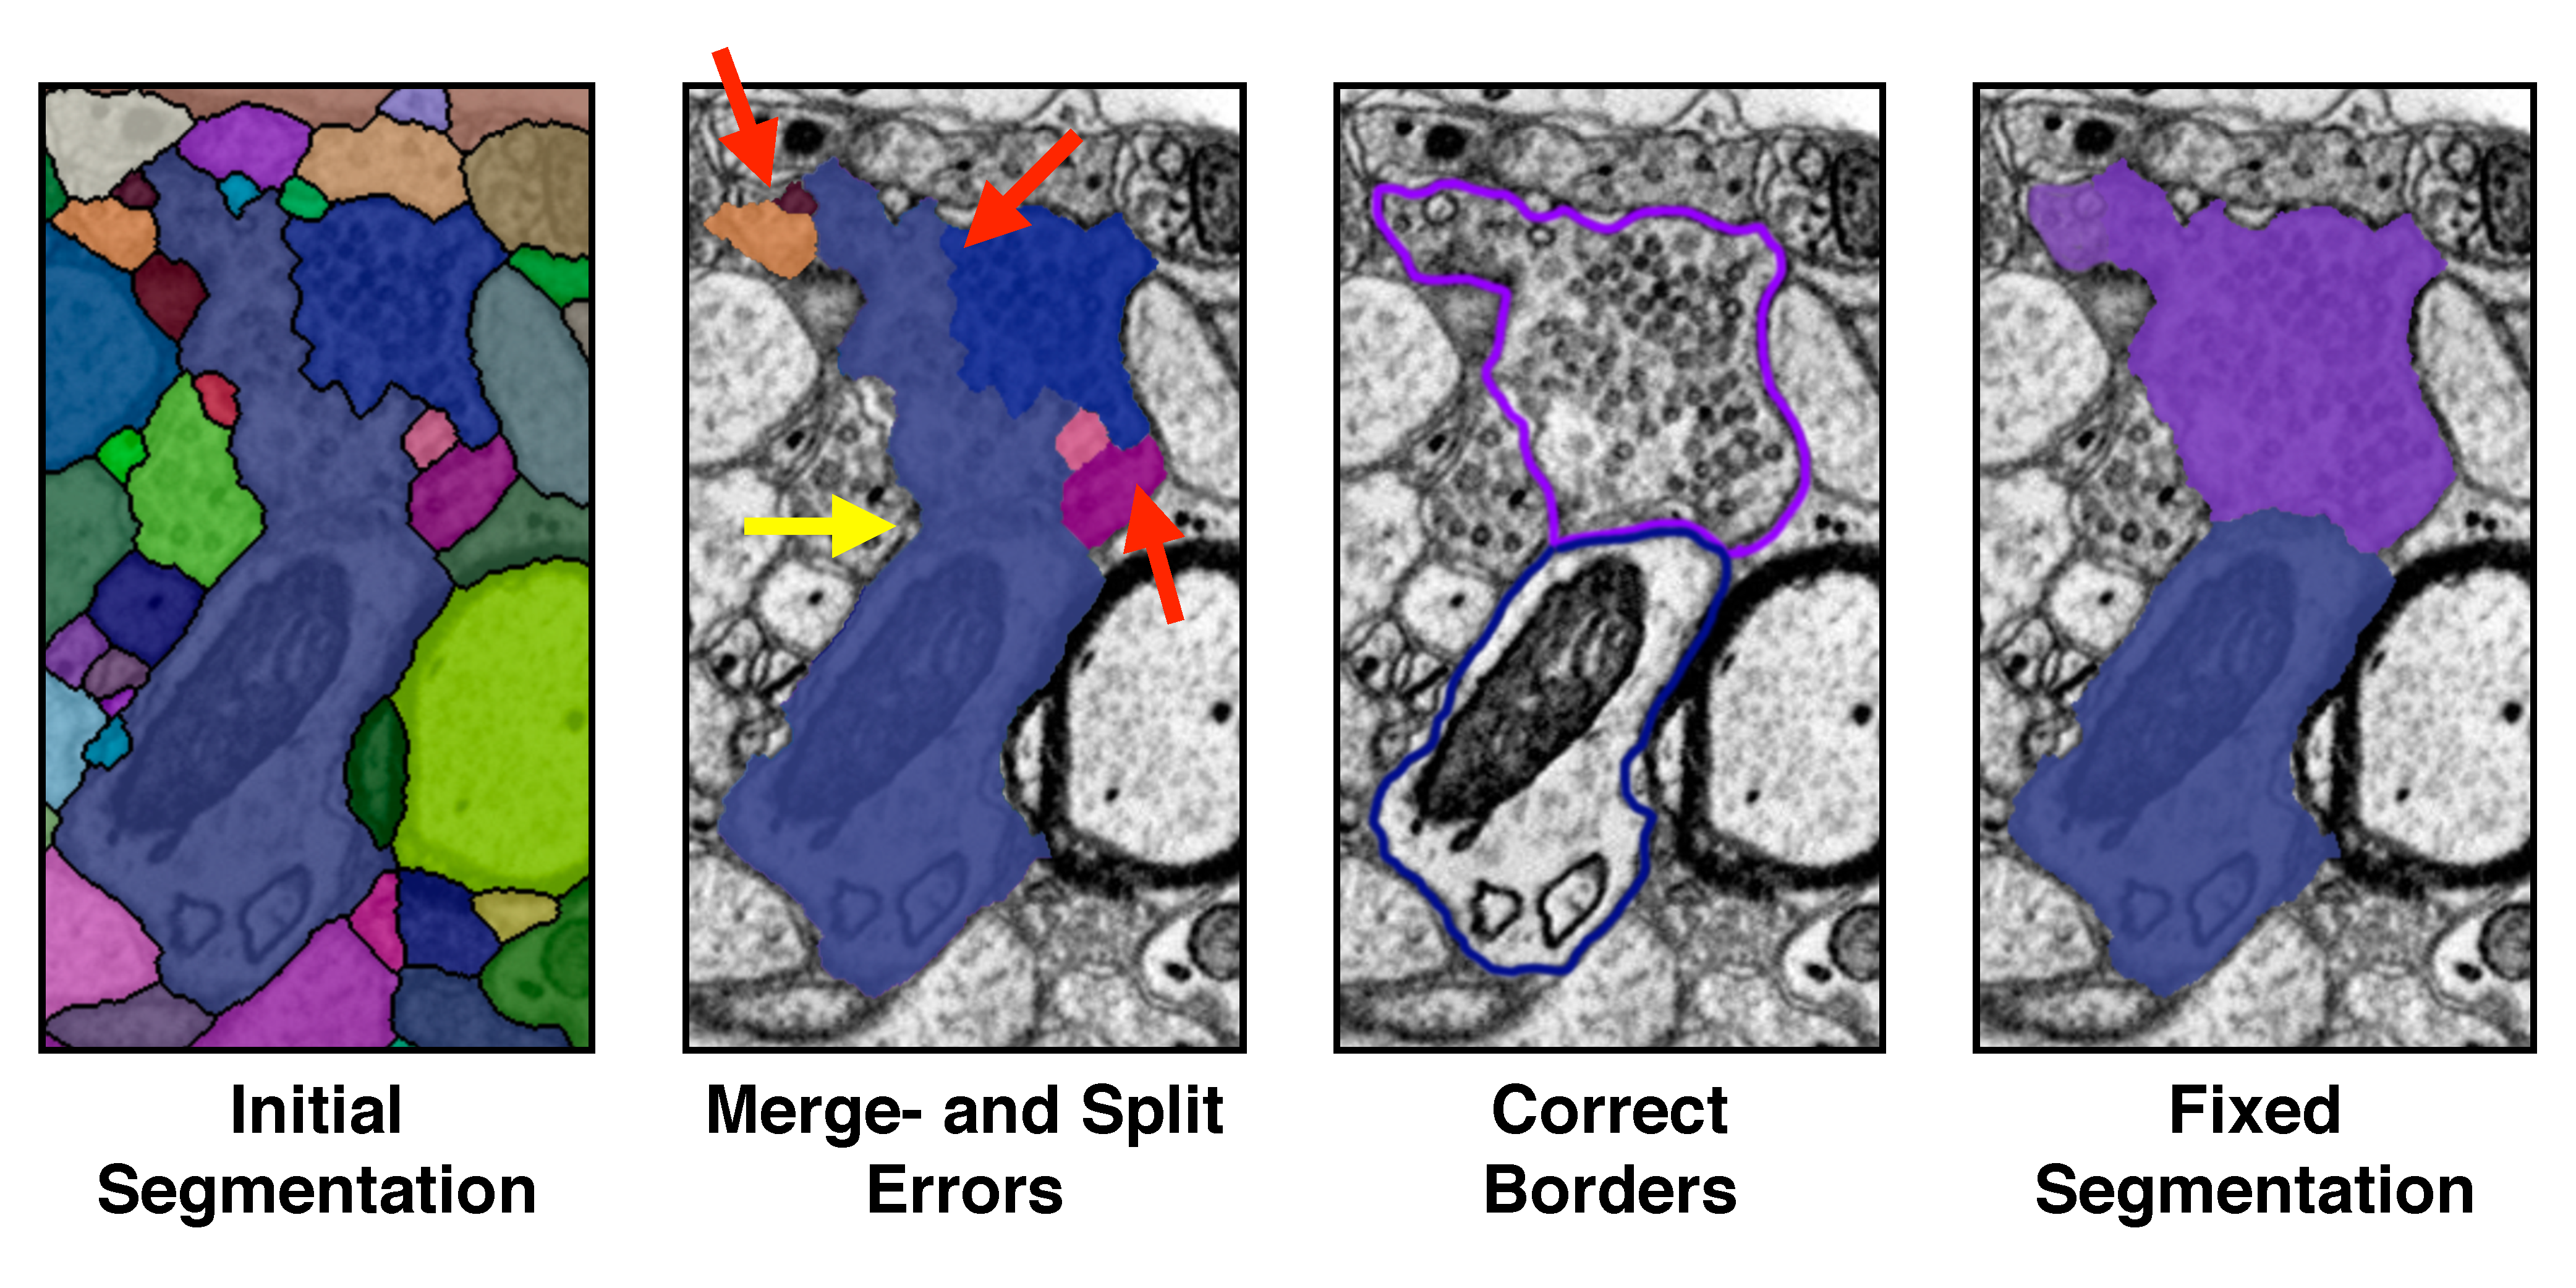
\includegraphics[width=\linewidth]{merge_and_split_errors.pdf}
\end{center}
\vspace{-4mm}
   \caption{The most common proofreading corrections are fixing split errors (red arrows) and merge errors (yellow arrow). A fixed segmentation matches the cell borders.}
\label{fig:merge_and_slit_errors}
\end{figure}

Our goal is to automatically detect potential split and merge errors to reduce visual
inspection time. Further, to reduce correction time, we propose
corrections to the user to accept or reject. We call this process \textit{guided
proofreading}.

We train a classifier for split error detection with a convolutional neural network
(CNN). This takes as input patches of membrane segmentation probabilities, cell
segmentation masks, and boundary masks, and outputs a split-probability score. As we
must process large data, this classifier only operates on cell boundaries, which
reduces computation over methods that analyze every pixel. For merge errors, we
invert and reuse the split classification network, and ask it to rate a
set of generated boundaries that hypothesize a split. 

Possible erroneous regions are sorted by their score, and a candidate correction is generated for each
region. Then, a user works through this list of regions and corrections. In a
forced choice setting, the user either selects a correction or skips it to
advance to the next region. In an automatic setting, errors with a high probability are automatically corrected first, given an appropriate
probability threshold, after which the user would take over. Finally, to test
the limits of performance, we create an oracle which only accepts corrections
that improve the segmentation, based on knowledge of the ground truth. This is
guided proofreading with a perfect user.

We evaluate these methods on multiple connectomics datasets. For the forced
choice setting, we perform a quantitative user study with 20 novice users who
have no previous experience of proofreading EM data. We ask participants to
proofread a small segmentation volume in a fixed time frame. In a
between-subjects design, we compare guided proofreading to the semi-automatic
\textit{focused proofreading} approach by Plaza~\cite{focused_proofreading}. In
addition, we compare against the manual interactive proofreading tool
\textit{Dojo} by Haehn~\etal~\cite{haehn_dojo_2014}. We also asked four domain
experts to use guided proofreading and focused proofreading for comparison.

This paper makes the following contributions.
%
First, we present a CNN-based boundary classifier for split errors, plus a merge
error classifier that inverts the split error classifier. This is used to
propose merge error corrections, removing the need to manually draw the missing
edge. These classifiers perform well without much training data, which is
expensive to collect for connectomics data.
%
Second, we developed a guided proofreading approach to correcting segmentation
volumes, and an assessment scenario comparing forced-choice interaction with
automatic and oracle proofreading.
%
Third, we present the results of a quantitative user study assessing
guided proofreading. Our method is able to reduce segmentation
error faster than state-of-the-art semi-automatic tools for both novice and
expert users.

Guided proofreading is applicable to all existing automatic segmentation methods that
produce a label map. As such, we believe that our approach is a promising
direction to proofread segmentations more efficiently and better tackle large
volumes of connectomics imagery.